%%
%% This is file `sample-xelatex.tex',
%% generated with the docstrip utility.
%%
%% The original source files were:
%%
%% samples.dtx  (with options: `sigconf')
%% 
%% IMPORTANT NOTICE:
%% 
%% For the copyright see the source file.
%% 
%% Any modified versions of this file must be renamed
%% with new filenames distinct from sample-xelatex.tex.
%% 
%% For distribution of the original source see the terms
%% for copying and modification in the file samples.dtx.
%% 
%% This generated file may be distributed as long as the
%% original source files, as listed above, are part of the
%% same distribution. (The sources need not necessarily be
%% in the same archive or directory.)
%%
%% The first command in your LaTeX source must be the \documentclass command.
\documentclass[sigchi]{acmart}

\usepackage{graphicx}
\usepackage{textgreek}
\usepackage{xcolor}
\usepackage{tabularx}
\usepackage{makecell}
% \usepackage[utf8]{inputenc}
% \usepackage[T1]{fontenc}


%%
%% \BibTeX command to typeset BibTeX logo in the docs
\AtBeginDocument{%
  \providecommand\BibTeX{{%
    \normalfont B\kern-0.5em{\scshape i\kern-0.25em b}\kern-0.8em\TeX}}}

\settopmatter{printacmref=false}
\settopmatter{printfolios=true}

%% Rights management information.  This information is sent to you
%% when you complete the rights form.  These commands have SAMPLE
%% values in them; it is your responsibility as an author to replace
%% the commands and values with those provided to you when you
%% complete the rights form.
\setcopyright{iw3c2w3g}
\copyrightyear{}
\acmYear{}
\acmDOI{}

%% These commands are for a PROCEEDINGS abstract or paper.
\acmConference[]{}{}{}
\acmBooktitle{}
\acmPrice{}
\acmISBN{}


%%
%% Submission ID.
%% Use this when submitting an article to a sponsored event. You'll
%% receive a unique submission ID from the organizers
%% of the event, and this ID should be used as the parameter to this command.
%%\acmSubmissionID{123-A56-BU3}

%%
%% The majority of ACM publications use numbered citations and
%% references.  The command \citestyle{authoryear} switches to the
%% "author year" style.
%%
%% If you are preparing content for an event
%% sponsored by ACM SIGGRAPH, you must use the "author year" style of
%% citations and references.
%% Uncommenting
%% the next command will enable that style.
%%\citestyle{acmauthoryear}

%%
%% end of the preamble, start of the body of the document source.
\begin{document}

%%
%% The "title" command has an optional parameter,
%% allowing the author to define a "short title" to be used in page headers.
\title{College Majors, Earnings, and Employability: A Visual Investigation}

%%
%% The "author" command and its associated commands are used to define
%% the authors and their affiliations.
%% Of note is the shared affiliation of the first two authors, and the
%% "authornote" and "authornotemark" commands
%% used to denote shared contribution to the research.
\author{David Kwan}
% \authornote{Both authors contributed equally to this research.}
\email{dkwan33@yorku.ca}
% \orcid{1234-5678-9012}
\affiliation{%
  \institution{York University}
  \streetaddress{4700 Keele St.}
  \city{Toronto}
  \state{Ontario}
  \postcode{M3J 1P3}
}

%%
%% By default, the full list of authors will be used in the page
%% headers. Often, this list is too long, and will overlap
%% other information printed in the page headers. This command allows
%% the author to define a more concise list
%% of authors' names for this purpose.
% \renewcommand{\shortauthors}{Trovato and Tobin, et al.}

%%
%% The abstract is a short summary of the work to be presented in the
%% article.
\begin{abstract}
 I present a novel series of visualizations created in Tableau for the purpose of investigating the earnings, employability, and gender wage gap between nearly all possible college majors and fields. Principles of visualization design are adhered to, and question-targeted interactive dashboards allow the user flexibility to control and investigate whatever relationships they desire. 
\end{abstract}

%%
%% The code below is generated by the tool at http://dl.acm.org/ccs.cfm.
%% Please copy and paste the code instead of the example below.
%%
% \begin{CCSXML}
% <ccs2012>
%  <concept>
%   <concept_id>10010520.10010553.10010562</concept_id>
%   <concept_desc>Computer systems organization~Embedded systems</concept_desc>
%   <concept_significance>500</concept_significance>
%  </concept>
%  <concept>
%   <concept_id>10010520.10010575.10010755</concept_id>
%   <concept_desc>Computer systems organization~Redundancy</concept_desc>
%   <concept_significance>300</concept_significance>
%  </concept>
%  <concept>
%   <concept_id>10010520.10010553.10010554</concept_id>
%   <concept_desc>Computer systems organization~Robotics</concept_desc>
%   <concept_significance>100</concept_significance>
%  </concept>
%  <concept>
%   <concept_id>10003033.10003083.10003095</concept_id>
%   <concept_desc>Networks~Network reliability</concept_desc>
%   <concept_significance>100</concept_significance>
%  </concept>
% </ccs2012>
% \end{CCSXML}

% \ccsdesc[500]{Computer systems organization~Embedded systems}
% \ccsdesc[300]{Computer systems organization~Redundancy}
% \ccsdesc{Computer systems organization~Robotics}
% \ccsdesc[100]{Networks~Network reliability}

%%
%% Keywords. The author(s) should pick words that accurately describe
%% the work being presented. Separate the keywords with commas.
% \keywords{data sets, neural networks, gaze detection, text tagging}

%% A "teaser" image appears between the author and affiliation
%% information and the body of the document, and typically spans the
%% page.
% \begin{teaserfigure}
%   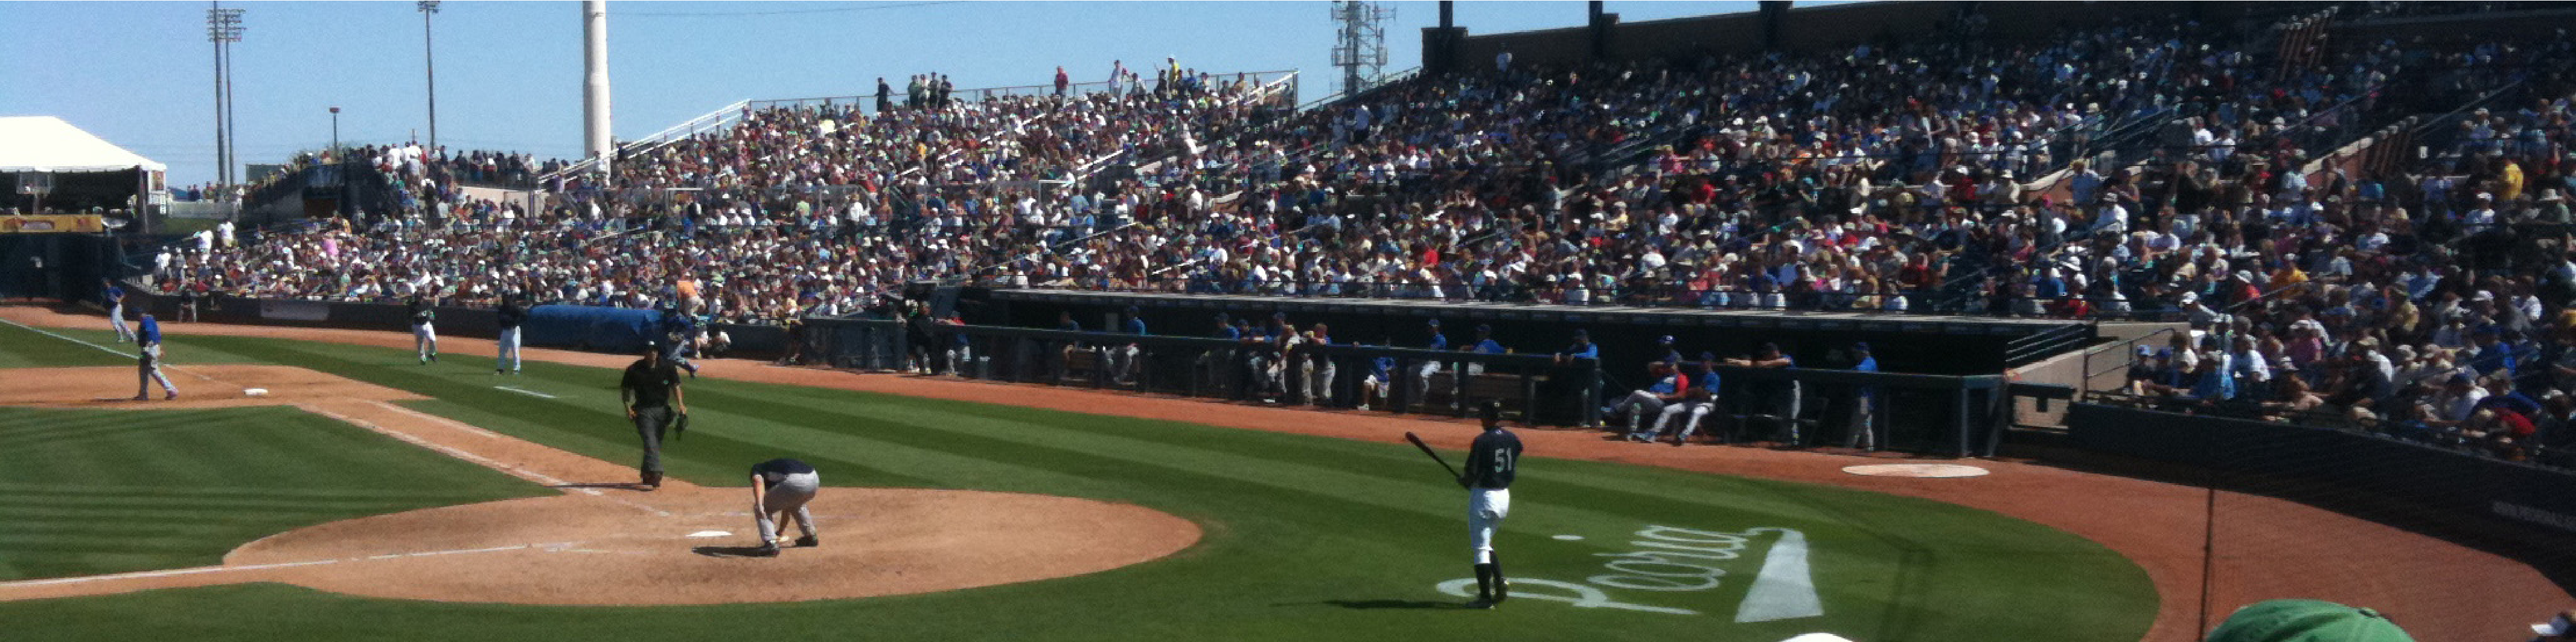
\includegraphics[width=\textwidth]{sampleteaser}
%   \caption{Seattle Mariners at Spring Training, 2010.}
%   \Description{Enjoying the baseball game from the third-base
%   seats. Ichiro Suzuki preparing to bat.}
%   \label{fig:teaser}
% \end{teaserfigure}

%%
%% This command processes the author and affiliation and title
%% information and builds the first part of the formatted document.
\maketitle

\section{Introduction}

For many students, perhaps almost every student, a major concern after graduation is employment. A college degree is by no means a guarantee of employment, nor is it a guarantee of economic safety, but it most certainly can help. The choice of major is a one of earliest decisions in a student's career, it can open many doors and offer many opportunities, but to many, the "wrong" choice may seem like a waste of time. After all, an unemployable or "useless" degree still takes just as much time as other degrees. There are a plethora of questions that prospective students, current students, or even recent graduates could be interested in: 
\begin{itemize}
\item{What kind of jobs are there?}
\item{What subjects are more popular?}
\item{What are students studying?}
\item{What do students specialize in?}
\item{Who makes more money?}
\item{Who is more employable?}
\item{Does the degree even matter?}
\end{itemize}
These are all valuable questions and are only a fraction of the possible questions regarding choice of college major. To that end, this investigation aims to answer all of the above and more using data visualization techniques with the Tableau software platform.

\section{Data Set}

In 2014, Ben Casselman wrote an article entitled \textit{The Economic Guide To Picking A College Major} published on the political and economic blog \textit{FiveThirtyEight} associated with ABC News \cite{fivethirtyeight}. This article used a full data set from the 2014 United States Census courtesy of the United States Census Bureau Public-Use Microdata. However, using this data set, Casselman only "ranked" the college majors in terms of earnings. Furthermore, Casselman did not create any data visualization. This is unfortunate as the data set itself holds much more potential. \textit{FiveThirtyEight} has made this data set public on Github (although the source was public to begin with, it is difficult to work with), along with the R script used to pull all the relevant data from the Census Bureau \cite{github}. 

The data itself is comprised of a few tables. The two most detailed contain data for recent graduates, being those of age 28 or less, as well as data pertaining to all ages. Each row pertains to a college major (e.g. Biomedical Engineering), and the first and foremost data column contains the broader major category (e.g. Engineering). Both of these are categorical data fields. The rest of the columns, of which there are many, are all quantitative. These data fields include the total number of people with that major, the total employed, the total unemployed, median salary of that major, gender, and much more. Data transformation was performed when required.

  \begin{figure*}[thpb]
  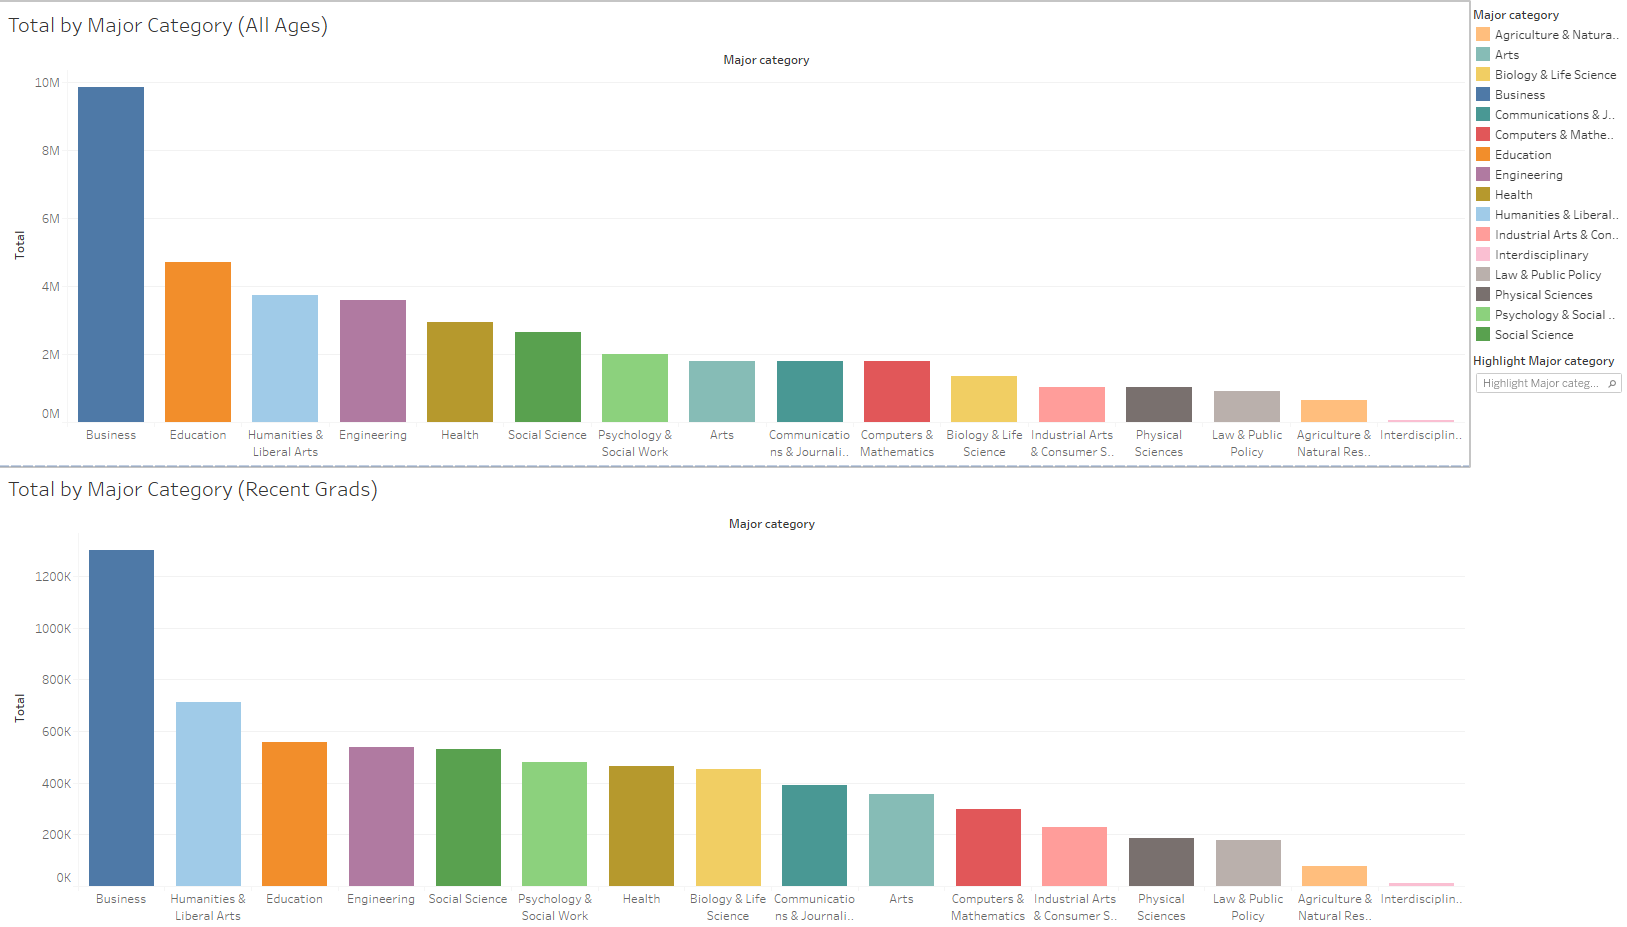
\includegraphics[width=1.0\textwidth]{DB1.png}
     \caption{Dashboard 1: Total Counts for each Major Category for both recent grads and all ages}
         \label{fig:db1}
  \end{figure*}
  
\section{Visualization Overview}

Using this data set, I have created a series of charts and dashboards using the Tableau platform. My focus is on recent graduates, so much of the data is from the recent graduates table, although data from the all-ages table are used as well whenever the comparison is worthwhile. 

The charts created include bar charts, box plots, scatterplots, and a map chart. Both the expressiveness and effectiveness principles of visualization design \cite{munzner} were adhered to as best as possible. Other available options such as packed-bubble charts were not chosen because it provided no clear advantage, even when placed on a dashboard with other types of charts. The map chart is a good example of a chart that, although does not strictly follow the expressiveness principle, had value especially when placed on a dashboard with interactivity.

Multiple dashboards were created with the goal of answering one or more specific questions that the user may have. All these dashboards provide value with interactive features, allowing the user to choose what they want to focus on. The interactivity cannot be shown here, nor is it particularly valuable to show screenshots of individual filters, but both filtering and highlighting can be done based on either major category or major specialization in all dashboards. Any filtering or highlighting done one chart of the dashboard updates all other charts on the dashboard. This was immensely important for this data set considering that there were 172 different majors to choose from. It is reasonable to expect that most users would only be interested in a few, or even one major specialization, and the corresponding major field, and thus would want to highlight or filter for the major that they wanted to investigate.

Furthermore, the dashboards provide juxtaposition between related graphs for comparison. One of the primary uses of juxtaposition in this case was to show a comparison between recent graduates and all ages along the same metrics. 

To avoid confusion in this paper, outside of the charts, "major" will be commonly referred to as "specialization", while "major category" will be commonly referred to as "field".

  \begin{figure*}[thpb]
  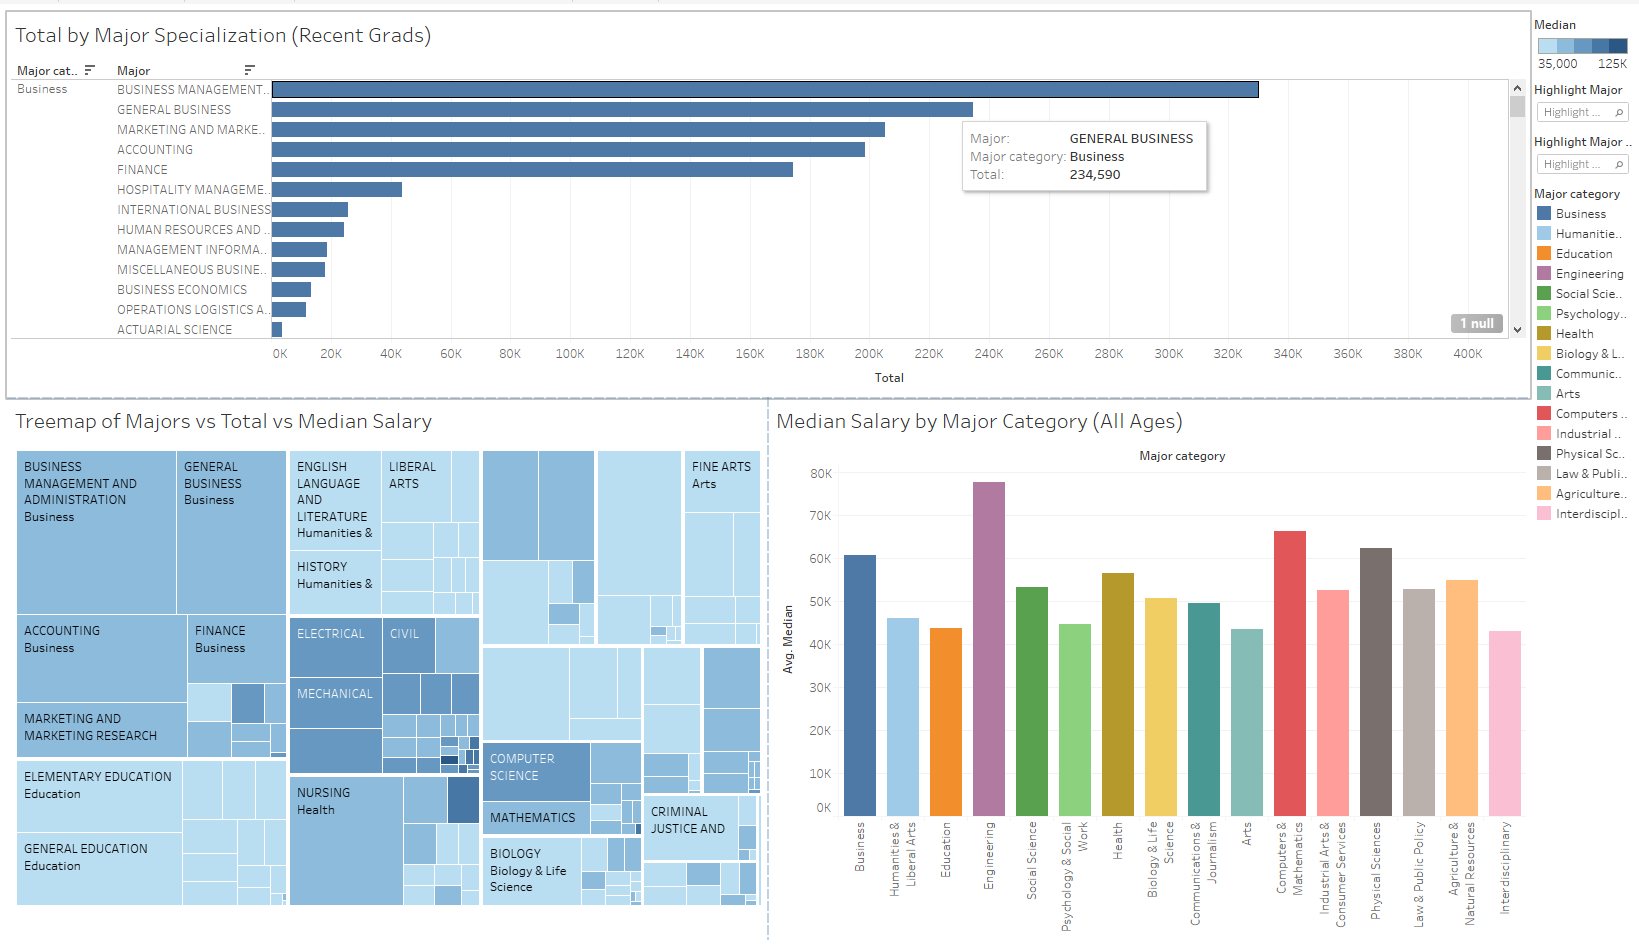
\includegraphics[width=1.0\textwidth]{DB2.png}
     \caption{Dashboard 2: Total Counts for each Major Specialization for recent grads juxtaposed with Treemap}
         \label{fig:db2}
  \end{figure*}
  
\section{Charts, Dashboards, Questions, and Answers}
\subsection{Dashboard 1: Fields and their Popularity}
\label{sec:db1}

Dashboard 1 shown in Fig. \ref{fig:db1} introduces the user to the data set, as it only shows the major categories and not the major specializations. Following the expressiveness and effectiveness principles, the bar charts here represent the quantitative variable (Total) as height, while the categorical variable (Major category) is represented with colour hue. It is important to note here that the colours used for the major categories here are used throughout all the visualizations. This is important of course, for consistency. Furthermore, the large number of categories here means many colour hues had to be used, which after a certain point can confuse the reader and be hard to distinguish from one another. This is an unfortunate drawback to my visualization solution, but cannot be avoided, as the major categories cannot be further group, nor would it be fair to eliminate any as a base filter. 

This dashboard answers the question "What kind of jobs are there?". For now, we can assume what people are studying is representative of the jobs that exist, although Dashboard 5 shows why this may not be the case when we look at under-utilization rate. It may be technically more accurate to say "What are people studying?" but that seems less pertinent to the intended reader. Clearly business is the dominant field in terms of popularity by a large margin. Physical sciences, Law, Agriculture are relatively unpopular. The juxtaposition of recent graduates vs all ages on this dashboard lets the reader infer if there are fields that are losing or gaining popularity. The most significant change seems to be a large increase in the current popularity of Biology and Life Science.


  \begin{figure*}[thpb]
  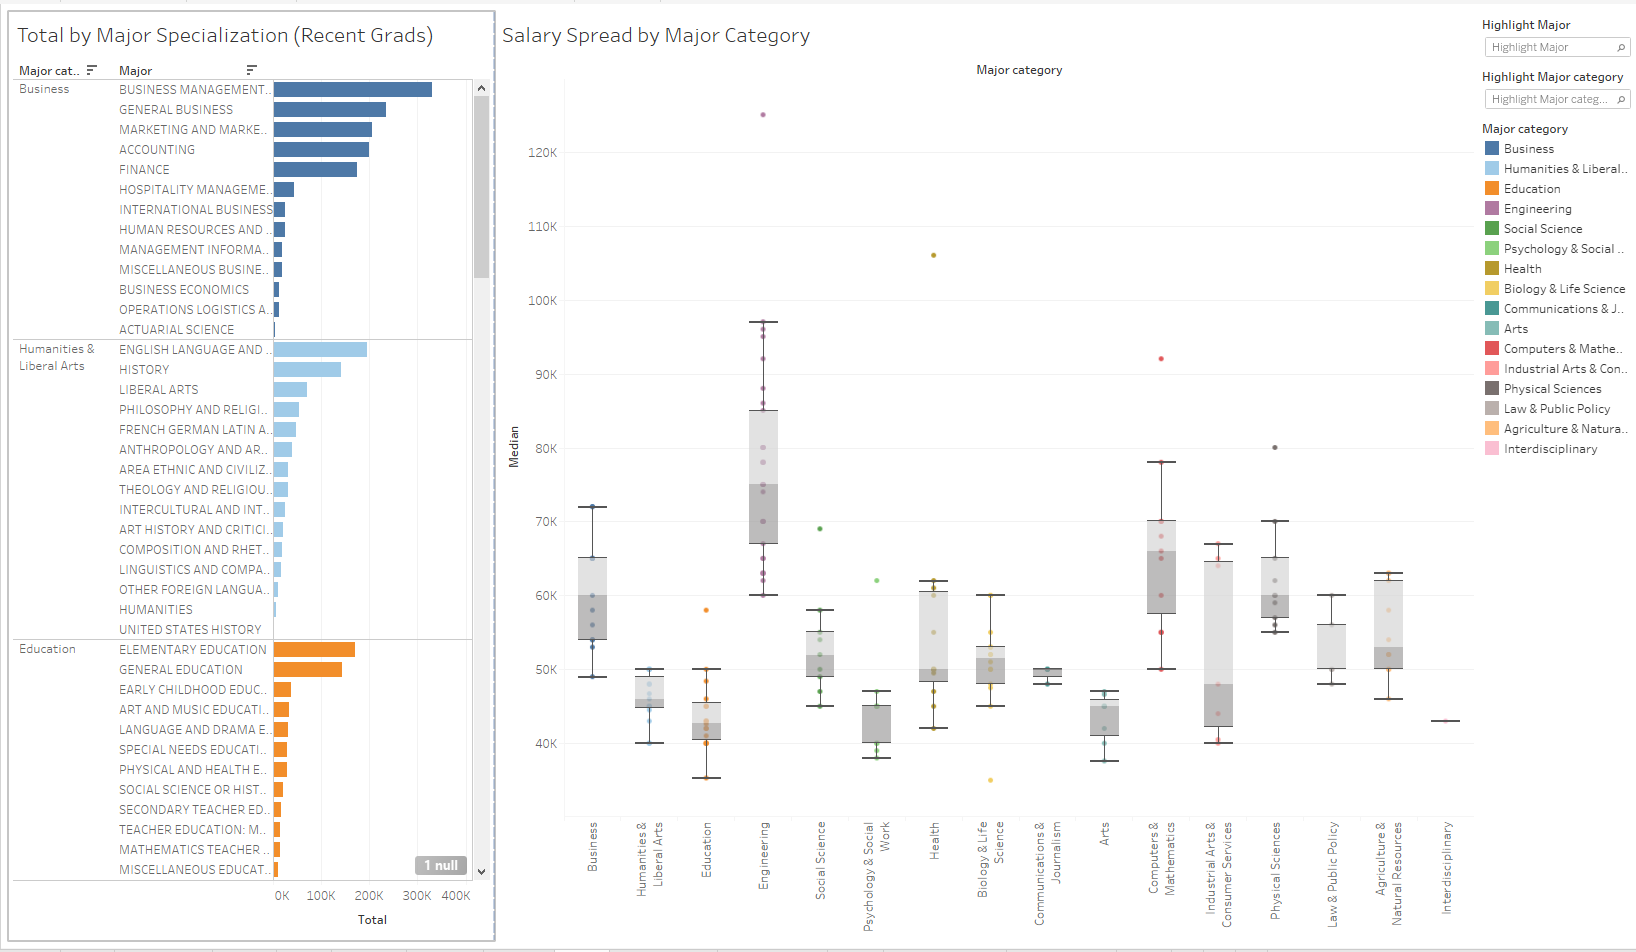
\includegraphics[width=1.0\textwidth]{DB3.png}
     \caption{Dashboard 3: Major Categories and a Box Plot of all Earnings for Majors and Major Categories}
         \label{fig:db3}
  \end{figure*}

\subsection{Dashboard 2: Specializations, Popularity, and an Introduction to Earnings}
\label{sec:db2}

The purpose of Dashboard 2 shown in Fig. \ref{fig:db2} is to, firstly, give the user an introduction to major specializations. Rather than showing the broader categories as in Fig. \ref{fig:db1}, we now show each field broken down into its individual specializations, and the total count for each specialization is given as well. Secondly, this dashboard serves to give the user a broad overview of earnings by field, as well as allow the user to at-a-glance look at earnings of interesting specializations. This dashboard was designed to answer the following questions: 
\begin{itemize}
\item{Which specializations are more popular?}
\item{Which specializations make less money than the rest of the field?  Which make more?}
\item{Which fields make more money?}
\end{itemize}

The first chart on Dashboard 2 is a grouped bar chart. This bar chart, similar to the charts on Dashboard 1, shows the total counts for each major specialization. Since there are 172 specializations, with approximately a dozen specializations per field, it is unreasonable to use a stacked bar chart. Furthermore, a grouped bar chart is more useful for comparing differences between the specializations themselves, as the user would be interested in comparing individual majors to other majors, such as Computer Science vs Computer and Information Systems. The grouped bar chart is allocated enough space on the dashboard to show one field at a time. The user can filter by major or major category to view whatever they are interested in. In this way, the problem of scale is addressed with filtering and highlighting. 

The second chart is map chart showing fields, their specializations, the total count encoded by area, and the salary encoded by colour saturation. Each field is the parent and each specialization is a node. Area and saturation do not strictly follow the expressiveness principle, but the map chart has many beneficial trade-offs. The map chart deals with scale significantly better than other charts, as it can fit all 172 majors on very little real-estate. It provides a good broad overview of the fields and can at a glance, due to pre-attentive processing \cite{munzner}, show any significant outliers within the region. It is easy for the user to identify which fields have higher earnings simply by how dark the region is. Any specializations within the field that are significantly lighter or significantly darker can be seen quickly by the user, and with a mouse-over tooltip, that specialization can be revealed. For example, the Pharmaceutical specialization within the Health field is significantly darker and thus has much higher earnings than the rest of the field. Similarly, Hospitality Management within the Business field is significantly lighter and thus has much lower earnings.

The third chart is bar chart showing the average earnings of each field. This is the same information shown by the saturation of the region in the map chart, but since saturation is a relatively poor encoding compared to height, this bar chart was included to give users a more clear picture of the earnings per field.

It is important to note that all portrayals of salary on this dashboard use the salary information for all ages rather than for recent graduates. This was done deliberately because the user, when looking at general salary information, is mostly interested in how much they \textit{can} make rather than how much they will make right out of school. Furthermore, the salary levels of recent graduates are very similar, and would have resulted in a map chart with mostly homogeneous colour. This extends to Dashboard 3 as well, but not to Dashboard 4, where the salary is clearly defined as either recent graduate or all ages, since the comparison between the two is what is important on that dashboard.

\begin{figure*}[thpb]
  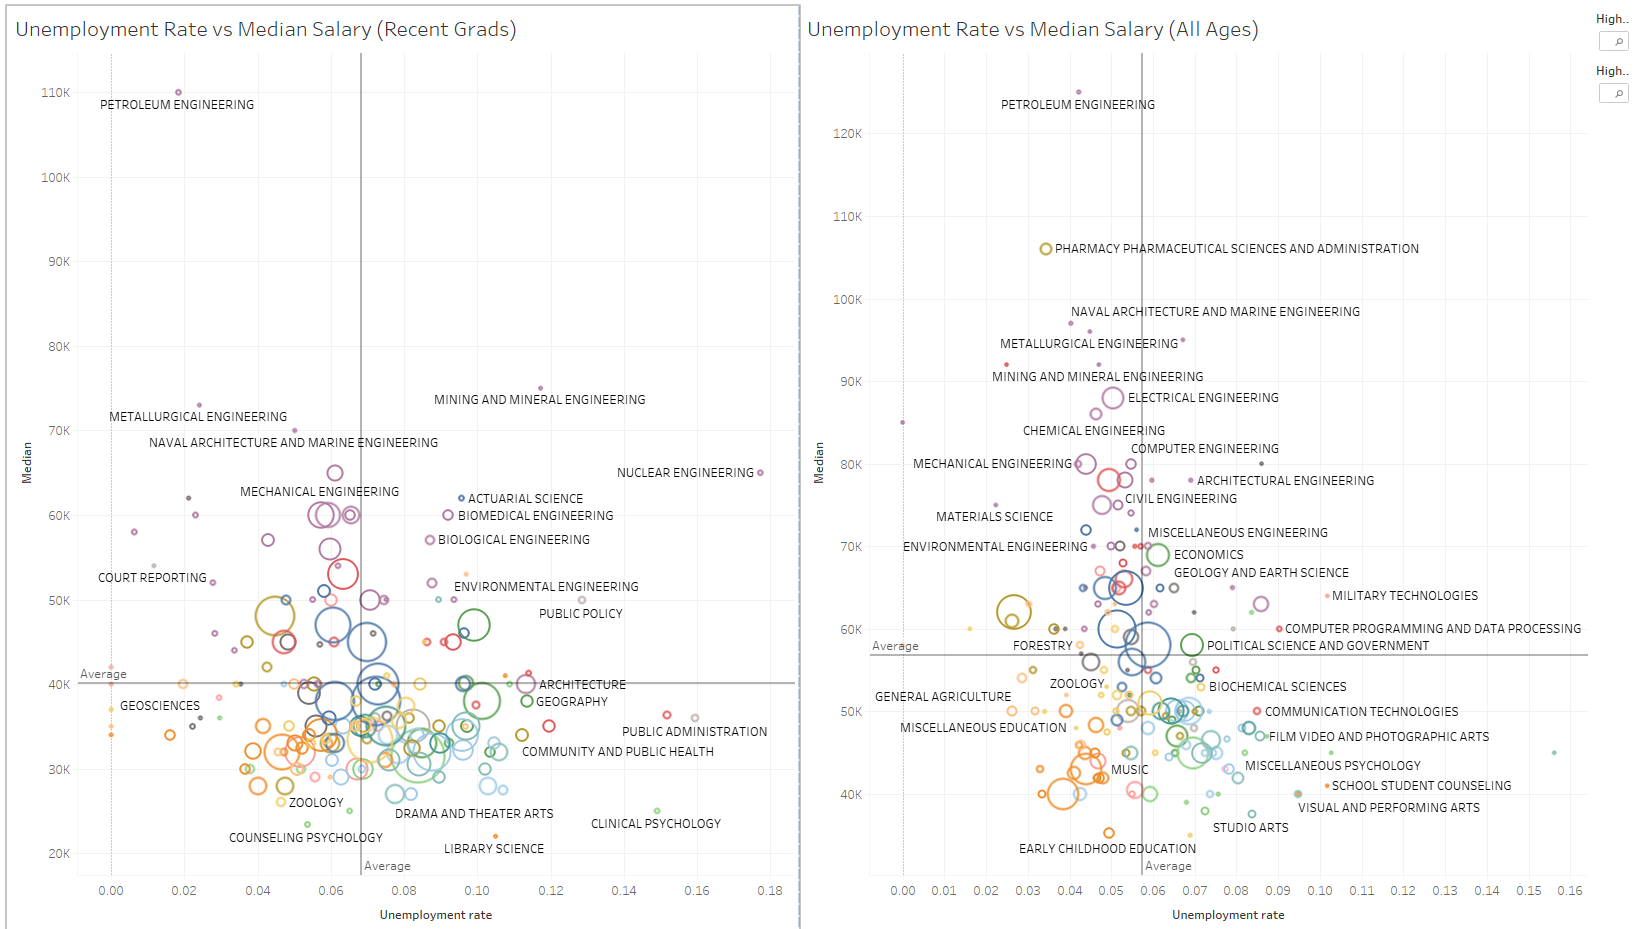
\includegraphics[width=1.0\textwidth]{DB4.png}
     \caption{Dashboard 4: Unemployment Rate vs Median Salary for recent grads and all ages}
         \label{fig:db4}
  \end{figure*}
  
\subsection{Dashboard 3: An In-Depth Look at Earnings}
\label{sec:db3}

Dashboard 3 shown in Fig. \ref{fig:db3} shows a much more in-depth overview of earnings. The primary focus here is the box plot of earnings for each field, with points (that can be highlighted or filtered) for each specialization. This dashboard is particularly useful for outlining the salary info of an individual specialization (using highlighting) and how it relates to other specializations, both within and outside the field. It is also useful for comparing with the median and quartiles of the field, to see where that specialization lies within the field itself. With this dashboard, the user can answer the following questions:
\begin{itemize}
\item{Which fields earn more? Which specializations?}
\item{What are the salary differences between fields? Between specializations?}
\item{What about between specializations within the same subject?}
\item{Does salary within a particular field vary much?}
\item{Are there specializations that make much more or much less than the field?}
\end{itemize}
A user can highlight a specific specialization they are interested in to bring up a tooltip with relevant information as well as to see where that point lies within the overall distribution. The box plot on this dashboard is effective at showing range and outliers. The range is valuable for seeing the spread of salaries within the field, and the outliers let you immediately see if there are specializations that make significantly more or less than the rest of the field. The map chart is dashboard 2 also showed this information, but that was encoded with colour saturation, and was thus not as effective as the height encoding here.

There are 7 positive outliers, some of the more notable ones include Petroleum Engineering in the field of Engineering, Pharmaceutical Sciences in the field of Health, and Economics in the field of Social Science. There is one negative outlier, quite a surprising one: Neuroscience in the field of Biology and Life Science.

The box plot on this dashboard has no been ordered based on salary. Instead, the same ordering from Dashboard 1 has been kept. This consistent ordering helps combat the colour encoding issue where we have too many colour hues for too many fields. In fact, this ordering is particularly important on the box plot because colour hue is hard to distinguish on the plot due to the small size of the marks.

  \begin{figure*}[thpb]
  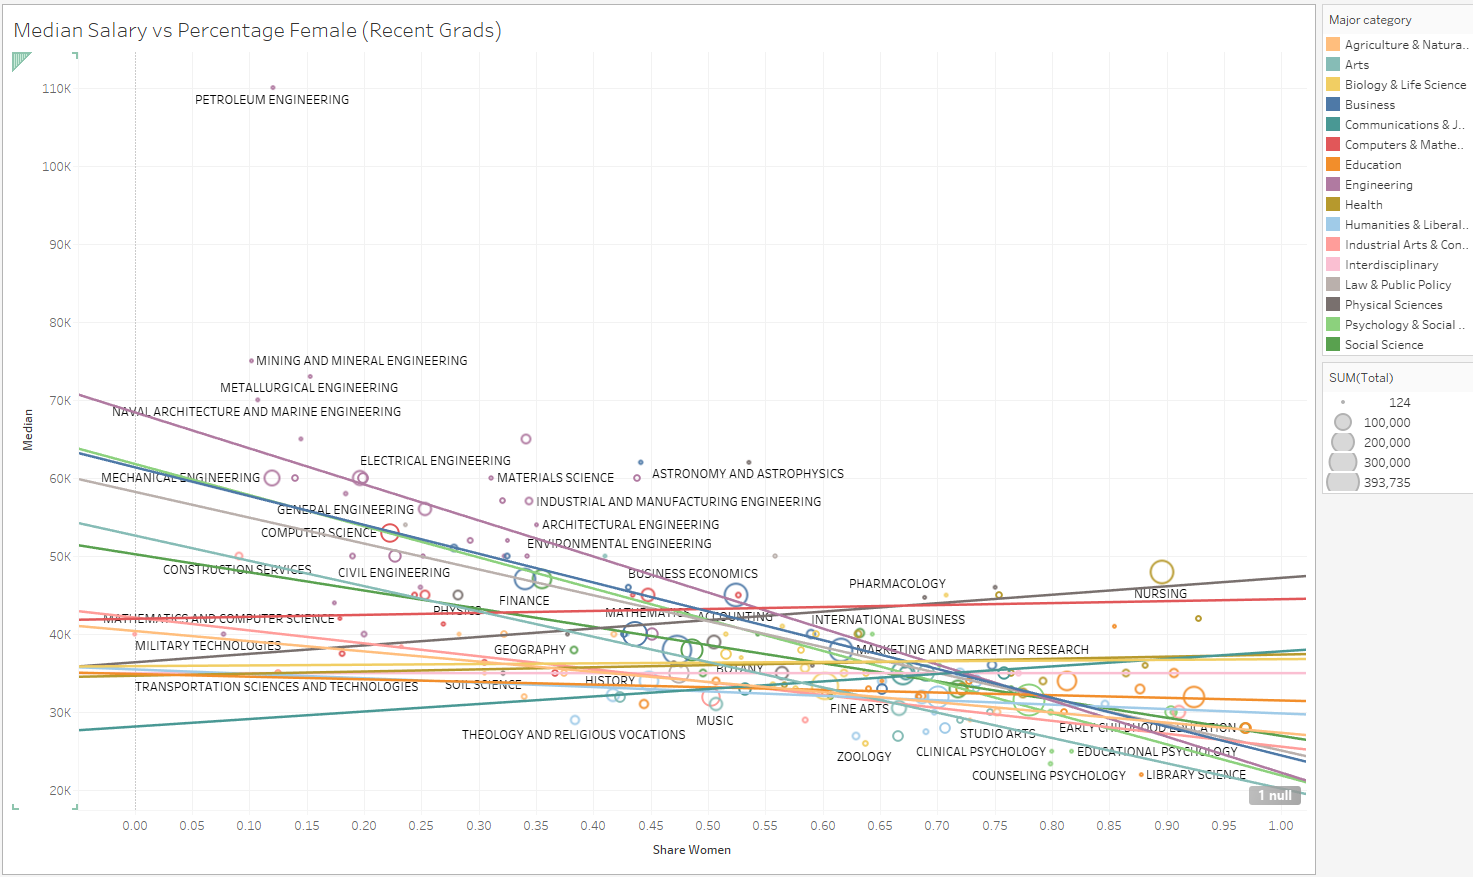
\includegraphics[width=1.0\textwidth]{SP1.png}
     \caption{Median Salary vs Percentage Female}
         \label{fig:sp1}
  \end{figure*}


\subsection{Dashboard 4: Earnings and Employability}
\label{sec:db4}

Dashboard 4 shown in Fig. \ref{fig:db4} allows the user to investigate employability. Furthermore, it specifically aims to investigate the difference between recent graduates and all ages. From this dashboard, the following questions can be answered:
\begin{itemize}
\item{Which specializations are more employable? How does this relate to earnings?}
\item{Does the employability for a specialization improve over time?}
\item{How does the employability for a specialization compare to other specializations?}
\item{Are there fields that are more employable or less employable?}
\end{itemize}
The dashboard shows two scatter plots. Each scatter plot shows the Unemployment Rate vs Median Salary for each specialization on the X and Y axes respectively. Colour hue, as-always, represents the field, and the size of each mark indicates the total count for the specialization. 

The averages for each quantitative variable are also shown as grey lines running through the plot to give the user a frame of reference for the centre. More importantly, it divides each plot into usable quadrants, from which the user quick inferences. By looking at any mark, the user can at a glance see which quadrant the mark lies in, and thus draw conclusions. Marks that lie in the upper-left quadrant are both high-earning and in demand. This quadrant is dominated by the field of Engineering (Purple), and to a lesser extent, the fields of Computers and Mathematics (Red) as well as Business (Dark Blue). Marks that lie in the bottom-right quadrant are both low-earning and in low demand. Here you can find mostly Humanities and Liberal Arts (Light Blue), as well as Psychology and Social Work (Light Green). The bottom-left and top-right quadrants are highly interesting. The bottom-left quadrant represents majors that are low-earning yet also in high demand. This quadrant is very clearly represented by the field of Education (Orange), and to a lesser extent, the field of Biology and Life Sciences (Yellow). 

The upper-right quadrant does not contain very many marks compared to the other three. Majors that lie here are both high-paying, yet also in low demand, which seems counter-intuitive at first. This is where the juxtaposition of the all ages graph is highly useful. As we can see, most of the marks that appear in this quadrant, such as Mining and Mineral Engineering, Nuclear Engineering, and Economics, have much lower unemployment than recent graduates. From this, we can infer that these specializations do not commonly employ recent graduates, and instead, prefer those that have experience. This makes a lot of sense especially when you consider the nature of the work of Nuclear Engineers or Economists.

  \begin{figure*}[thpb]
  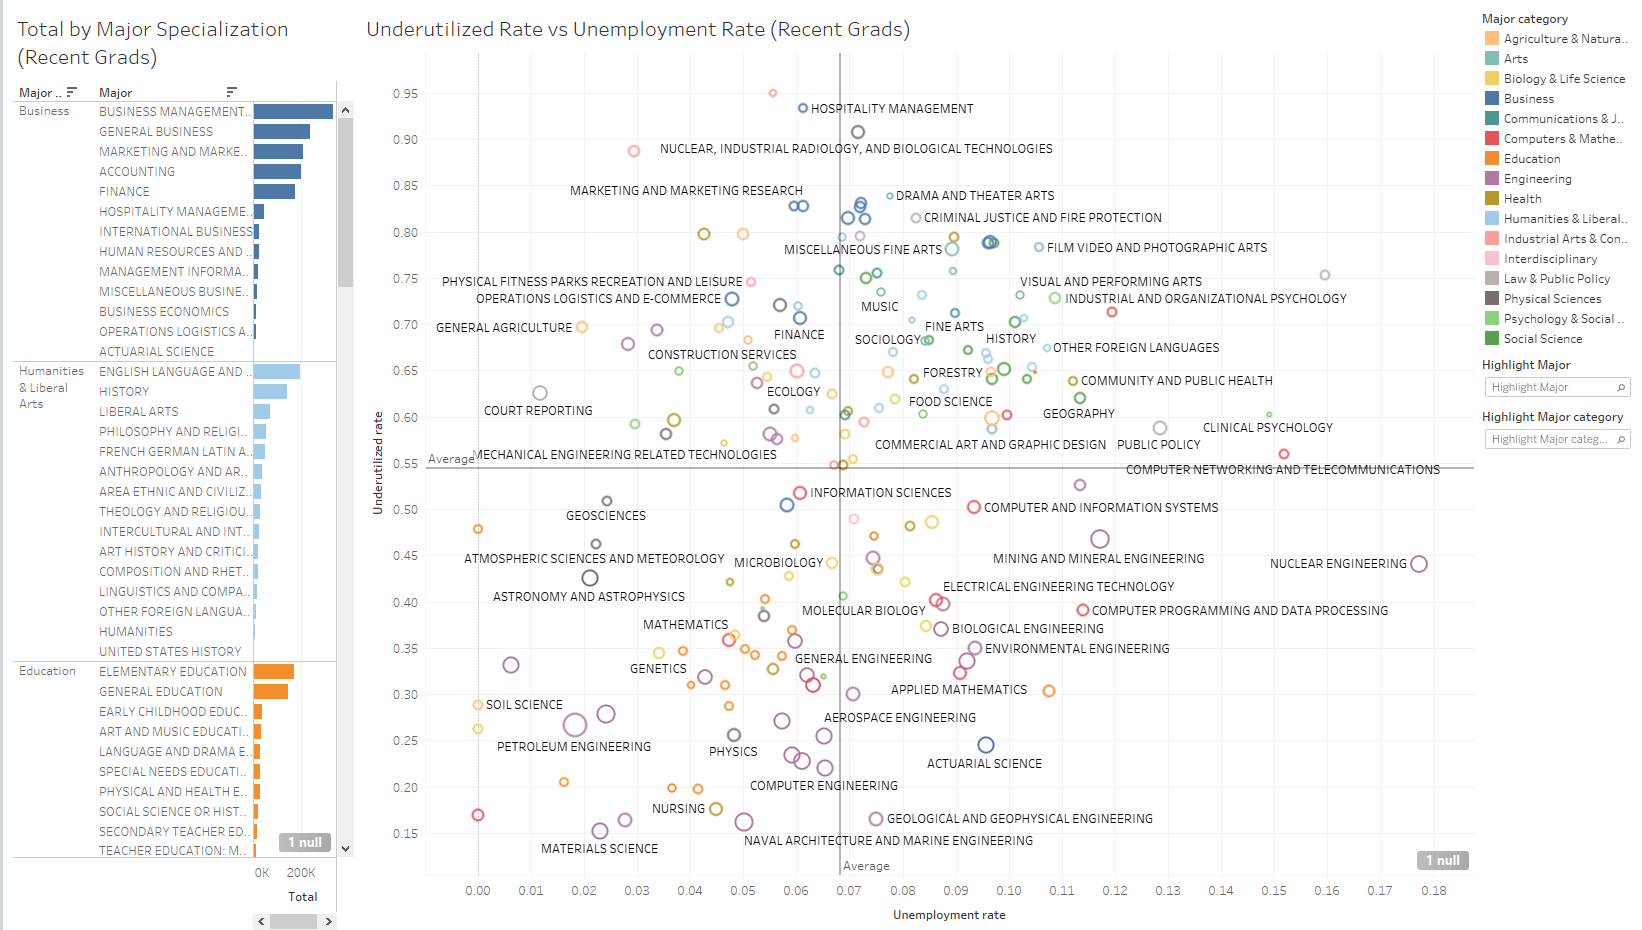
\includegraphics[width=1.0\textwidth]{DB5.png}
     \caption{Dashboard 5: Underutilized Rate vs Unemployment Rate}
         \label{fig:db5}
  \end{figure*}



\subsection{Earnings vs. Gender}
\label{sec:earningsgender}

Figure \ref{fig:sp1} displays a scatter plot showing salary vs the percentage of women with that major. This was not added to any dashboard as it is not particularly useful when juxtaposed with other graphs, since it already displays the two metrics that users are interested in when discussing this topic: the gender wage gap. The purpose of this chart is to investigate the following:
\begin{itemize}
\item{How does gender relate to salary?}
\item{Do different fields have different gender-wage gaps compared to others?}
\end{itemize}
The main focus of this scatter plot is the trend lines. Unlike the previous scatter plots on Fig. \ref{fig:db4}, the overall trend is in-fact, the primary thing the user wishes to see. For the most part, all the trend lines are either negatively correlated, or neutral. From this we can infer that the in general, a higher percentage of women is correlated with a lower salary, but this is different depending on the field. We can see that some fields have very steep negative correlations, such as Engineering and Business, while others, such as Education or Biology and Life Sciences are relatively neutral. Interestingly enough, and perhaps surprisingly, the field of Computers and Mathematics has a positive correlation.


\subsection{Dashboard 5: An In-Depth Look at Employability}
\label{sec:db5}

So far, many of our observations have been based on the assumption that the total count of those with a specific college major represents the number of jobs for the major. This is true for most, but for many, may not be an accurate assumption at all. To investigate this, I created a transformed data field that I have called "Underutilized Rate". The equation for the underutilized rate is as follows:
\begin{displaymath}
  \frac{(NonCollegeJobs + LowWageJobs)}{(NonCollegeJobs + LowWageJobs + CollegeJobs)}
\end{displaymath}
Effectively, the underutilized rate shows the number of those who are working jobs that do not actually utilize a college degree. It is important to note that due to limitations in the data set, it is not the under-utilization of that specific degree since census data does not exist for whether or not a job requires their college degree specifically; only whether or not they have a degree at all. However, it is likely safe to assume that it representative nonetheless, after all, school is simply the first building block in the career.

Dashboard 5 shown in Fig. \ref{fig:db5} shows a scatter plot of the underutilized rate vs unemployment rate for recent graduates. The grouped bar chart showing major specializations is present as well, to make it easier for the user to filer for their field or specialization of interest. It is important to note here that, unlike all the previous scatter plots, the size encoding does not encode total count but rather salary. This was done because the grouped bar chart already shows total count quite effectively, and so it would have been redundant to show it again as a size encoding on the scatter plot. Instead we show salary information since it is not present anywhere else on the dashboard, and, following the effectiveness principle, it is encoded with size since it is not the primary or even secondary metric that we are interested in.

This dashboard allows the user to answer the following questions:
\begin{itemize}
\item{Are degrees useful?}
\item{Which degrees are more useful than others?}
\item{Is a field or specialization possibly over-saturated?}
\item{Are there salary differences due to over-saturation?}
\end{itemize}

Similar to Dashboard 4, mean lines on the scatter plot provide a measure of centre and also split the plot into easy-to-discern quadrants. Marks that lie in the lower-left quadrant represent specializations that are both employed and utilized. Conversely, marks that lie in the upper-right quadrant represent specializations that have both low employment and are underutilized. Marks that lie in the bottom-right quadrant are utilized, but not employed. The specializations that are found here, such as Nuclear Engineering, seem to be similar to those found in the upper-right quadrant of Dashboard 4: indicating fields that are highly-specialized and require experience. Perhaps many of those with these degrees are still pursuing higher education such as doctorate degrees. Marks that lie in the upper-left quadrant are perhaps the most interesting on this dashboard. The specializations found here are highly employed but are underutilized. Specializations such as "Medical Assisting Services" and "Operations Logistics and E-commerce" are perhaps, at least according to this analysis, not particularly useful.

\section{Future Work and Conclusion}
In the future I would like improve this visualization by adding animation, especially if time-scale data could be made available and integrated with the current data. In Dashboard 4, where the changes in both earnings and employability can be seen, is in my opinion the most valuable dashboard and yet relatively cluttered. It is easy to miss certain interesting finds if you do not specifically filter for it. For example, the Pharmaceutical Sciences specialization makes a massive jump where it "shoots" from the lower left quadrant on the recent graduates chart all the way up to the 2nd-highest earning specialization on the all ages chart.

In conclusion, I have presented a series of interactive visualizations intended for prospective students, current students, and recent graduates to make informed decisions about their future. Many common questions regarding the earnings and employability of 172 college majors can be answered from these dashboards, and I have made it clear which dashboards are effective at answering which questions. A countless number of conclusions can be drawn from this data, and I have made a few of the most interesting observations within section 4. Further observations can be investigated at the users' pleasure, and I am sure many more conclusions can be made regarding the earnings and employability of various fields and specializations. 


% \section{Citations and Bibliographies}

% The use of \BibTeX\ for the preparation and formatting of one's
% references is strongly recommended. Authors' names should be complete
% --- use full first names (``Donald E. Knuth'') not initials
% (``D. E. Knuth'') --- and the salient identifying features of a
% reference should be included: title, year, volume, number, pages,
% article DOI, etc.

% The bibliography is included in your source document with these two
% commands, placed just before the \verb|\end{document}| command:
% \begin{verbatim}
%   \bibliographystyle{ACM-Reference-Format}
%   \bibliography{bibfile}
% \end{verbatim}
% where ``\verb|bibfile|'' is the name, without the ``\verb|.bib|''
% suffix, of the \BibTeX\ file.

% Citations and references are numbered by default. A small number of
% ACM publications have citations and references formatted in the
% ``author year'' style; for these exceptions, please include this
% command in the {\bfseries preamble} (before
% ``\verb|\begin{document}|'') of your \LaTeX\ source:
% \begin{verbatim}
%   \citestyle{acmauthoryear}
% \end{verbatim}

%   Some examples.  A paginated journal article \cite{Abril07}, an
%   enumerated journal article \cite{Cohen07}, a reference to an entire
%   issue \cite{JCohen96}, a monograph (whole book) \cite{Kosiur01}, a
%   monograph/whole book in a series (see 2a in spec. document)
%   \cite{Harel79}, a divisible-book such as an anthology or compilation
%   \cite{Editor00} followed by the same example, however we only output
%   the series if the volume number is given \cite{Editor00a} (so
%   Editor00a's series should NOT be present since it has no vol. no.),
%   a chapter in a divisible book \cite{Spector90}, a chapter in a
%   divisible book in a series \cite{Douglass98}, a multi-volume work as
%   book \cite{Knuth97}, an article in a proceedings (of a conference,
%   symposium, workshop for example) (paginated proceedings article)
%   \cite{Andler79}, a proceedings article with all possible elements
%   \cite{Smith10}, an example of an enumerated proceedings article
%   \cite{VanGundy07}, an informally published work \cite{Harel78}, a
%   doctoral dissertation \cite{Clarkson85}, a master's thesis:
%   \cite{anisi03}, an online document / world wide web resource
%   \cite{Thornburg01, Ablamowicz07, Poker06}, a video game (Case 1)
%   \cite{Obama08} and (Case 2) \cite{Novak03} and \cite{Lee05} and
%   (Case 3) a patent \cite{JoeScientist001}, work accepted for
%   publication \cite{rous08}, 'YYYYb'-test for prolific author
%   \cite{SaeediMEJ10} and \cite{SaeediJETC10}. Other cites might
%   contain 'duplicate' DOI and URLs (some SIAM articles)
%   \cite{Kirschmer:2010:AEI:1958016.1958018}. Boris / Barbara Beeton:
%   multi-volume works as books \cite{MR781536} and \cite{MR781537}. A
%   couple of citations with DOIs:
%   \cite{2004:ITE:1009386.1010128,Kirschmer:2010:AEI:1958016.1958018}. Online
%   citations: \cite{TUGInstmem, Thornburg01, CTANacmart}. Artifacts:
%   \cite{R} and \cite{UMassCitations}.

% \section{Acknowledgments}

% Identification of funding sources and other support, and thanks to
% individuals and groups that assisted in the research and the
% preparation of the work should be included in an acknowledgment
% section, which is placed just before the reference section in your
% document.

% This section has a special environment:
% \begin{verbatim}
%   \begin{acks}
%   ...
%   \end{acks}
% \end{verbatim}
% so that the information contained therein can be more easily collected
% during the article metadata extraction phase, and to ensure
% consistency in the spelling of the section heading.

% Authors should not prepare this section as a numbered or unnumbered {\verb|\section|}; please use the ``{\verb|acks|}'' environment.

% \section{Appendices}

% If your work needs an appendix, add it before the
% ``\verb|\end{document}|'' command at the conclusion of your source
% document.

% Start the appendix with the ``\verb|appendix|'' command:
% \begin{verbatim}
%   \appendix
% \end{verbatim}
% and note that in the appendix, sections are lettered, not
% numbered. This document has two appendices, demonstrating the section
% and subsection identification method.

% \section{SIGCHI Extended Abstracts}

% The ``\verb|sigchi-a|'' template style (available only in \LaTeX\ and
% not in Word) produces a landscape-orientation formatted article, with
% a wide left margin. Three environments are available for use with the
% ``\verb|sigchi-a|'' template style, and produce formatted output in
% the margin:
% \begin{itemize}
% \item {\verb|sidebar|}:  Place formatted text in the margin.
% \item {\verb|marginfigure|}: Place a figure in the margin.
% \item {\verb|margintable|}: Place a table in the margin.
% \end{itemize}

%%
%% The acknowledgments section is defined using the "acks" environment
%% (and NOT an unnumbered section). This ensures the proper
%% identification of the section in the article metadata, and the
%% consistent spelling of the heading.
% \begin{acks}
% To Robert, for the bagels and explaining CMYK and color spaces.
% \end{acks}

%%
%% The next two lines define the bibliography style to be used, and
%% the bibliography file.
\bibliographystyle{ACM-Reference-Format}
\bibliography{sample-base}

%%
%% If your work has an appendix, this is the place to put it.
% \appendix

% \section{Research Methods}

% \subsection{Part One}

% Lorem ipsum dolor sit amet, consectetur adipiscing elit. Morbi
% malesuada, quam in pulvinar varius, metus nunc fermentum urna, id
% sollicitudin purus odio sit amet enim. Aliquam ullamcorper eu ipsum
% vel mollis. Curabitur quis dictum nisl. Phasellus vel semper risus, et
% lacinia dolor. Integer ultricies commodo sem nec semper.

% \subsection{Part Two}

% Etiam commodo feugiat nisl pulvinar pellentesque. Etiam auctor sodales
% ligula, non varius nibh pulvinar semper. Suspendisse nec lectus non
% ipsum convallis congue hendrerit vitae sapien. Donec at laoreet
% eros. Vivamus non purus placerat, scelerisque diam eu, cursus
% ante. Etiam aliquam tortor auctor efficitur mattis.

% \section{Online Resources}

% Nam id fermentum dui. Suspendisse sagittis tortor a nulla mollis, in
% pulvinar ex pretium. Sed interdum orci quis metus euismod, et sagittis
% enim maximus. Vestibulum gravida massa ut felis suscipit
% congue. Quisque mattis elit a risus ultrices commodo venenatis eget
% dui. Etiam sagittis eleifend elementum.

% Nam interdum magna at lectus dignissim, ac dignissim lorem
% rhoncus. Maecenas eu arcu ac neque placerat aliquam. Nunc pulvinar
% massa et mattis lacinia.

\end{document}
\endinput
%%
%% End of file `sample-xelatex.tex'.
